\documentclass[utf8, 14pt, bold]{G7-32}
\sloppy

% Настройки стиля ГОСТ 7-32
% Для начала определяем, хотим мы или нет, чтобы рисунки и таблицы нумеровались в пределах раздела, или нам нужна сквозная нумерация.
% \EqInChapter % формулы будут нумероваться в пределах раздела
% \TableInChapter % таблицы будут нумероваться в пределах раздела
% \PicInChapter % рисунки будут нумероваться в пределах раздела

% Добавляем гипертекстовое оглавление в PDF
\usepackage[
  bookmarks=true, colorlinks=true, unicode=true,
  urlcolor=black,linkcolor=black, anchorcolor=black,
  citecolor=black, menucolor=black, filecolor=black,
]{hyperref}

\AfterHyperrefFix

\usepackage{microtype}% полезный пакет для микротипографии, увы под xelatex мало чего умеет, но под pdflatex хорошо улучшает читаемость

% Тире могут быть невидимы в Adobe Reader
\ifInvisibleDashes
  \MakeDashesBold
\fi
\usepackage{changepage}
\usepackage{graphicx}   % Пакет для включения рисунков

% С такими оно полями оно работает по-умолчанию:
% \RequirePackage[left=20mm,right=10mm,top=20mm,bottom=20mm,headsep=0pt,includefoot]{geometry}
% Если вас тошнит от поля в 10мм --- увеличивайте до 20-ти, ну и про переплёт не забывайте:
\geometry{right=10mm}
\geometry{left=30mm}
\geometry{bottom=20mm}
\geometry{ignorefoot}% считать от нижней границы текста


% Пакет Tikz
\usepackage{tikz}
\usetikzlibrary{arrows,positioning,shadows}

% Произвольная нумерация списков.
\usepackage{enumerate}

% ячейки в несколько строчек
\usepackage{multirow}

% itemize внутри tabular
\usepackage{paralist,array}

%\setlength{\parskip}{1ex plus0.5ex minus0.5ex} % разрыв между абзацами
\setlength{\parskip}{1ex} % разрыв между абзацами
\usepackage{blindtext}

% Центрирование подписей к плавающим окружениям
%\usepackage[justification=centering]{caption}

\usepackage{newfloat}
\DeclareFloatingEnvironment[
  placement={!ht},
  name=Equation
]{eqndescNoIndent}
\edef\fixEqndesc{\noexpand\setlength{\noexpand\parindent}{\the\parindent}\noexpand\setlength{\noexpand\parskip}{\the\parskip}}
\newenvironment{eqndesc}[1][!ht]{%
  \begin{eqndescNoIndent}[#1]%
    \fixEqndesc%
    }
    {\end{eqndescNoIndent}}

\makeatletter
\def\thenomenclature{%
  \if@intoc\addcontentsline{toc}{section}{\nomname}\fi%
  \nompreamble
  \list{}{%
    \labelwidth\nom@tempdim
    \leftmargin\labelwidth
    \advance\leftmargin\labelsep
    \itemsep\nomitemsep
    \let\makelabel\nomlabel}
}
\makeatother

\usepackage{array, booktabs, hhline, tabularx, indentfirst, calc, textcase, xstring}
\usepackage{stackrel}
\usepackage{ulem}
\usepackage{adjustbox}

\usepackage{algorithm}
\usepackage{algpseudocode}
\usepackage{titlesec}
\usepackage{wrapfig}
% 8 Листинги

\usepackage{listings}

% Значения по умолчанию
\lstset{
  basicstyle= \footnotesize,
  breakatwhitespace=true,% разрыв строк только на whitespacce
  breaklines=true,       % переносить длинные строки
%   captionpos=b,          % подписи снизу -- вроде не надо
  inputencoding=koi8-r,
  numbers=left,          % нумерация слева
  numberstyle=\footnotesize,
  showspaces=false,      % показывать пробелы подчеркиваниями -- идиотизм 70-х годов
  showstringspaces=false,
  showtabs=false,        % и табы тоже
  stepnumber=1,
  tabsize=4,              % кому нужны табы по 8 символов?
  frame=single
}

% Стиль для псевдокода: строчки обычно короткие, поэтому размер шрифта побольше
\lstdefinestyle{pseudocode}{
  basicstyle=\small,
  keywordstyle=\color{black}\bfseries\underbar,
  language=Pseudocode,
  numberstyle=\footnotesize,
  commentstyle=\footnotesize\it
}

% Стиль для обычного кода: маленький шрифт
\lstdefinestyle{realcode}{
  basicstyle=\scriptsize,
  numberstyle=\footnotesize
}

% Стиль для коротких кусков обычного кода: средний шрифт
\lstdefinestyle{simplecode}{
  basicstyle=\footnotesize,
  numberstyle=\footnotesize
}

% Стиль для BNF
\lstdefinestyle{grammar}{
  basicstyle=\footnotesize,
  numberstyle=\footnotesize,
  stringstyle=\bfseries\ttfamily,
  language=BNF
}

% Определим свой язык для написания псевдокодов на основе Python
\lstdefinelanguage[]{Pseudocode}[]{Python}{
  morekeywords={each,empty,wait,do},% ключевые слова добавлять сюда
  morecomment=[s]{\{}{\}},% комменты {а-ля Pascal} смотрятся нагляднее
  literate=% а сюда добавлять операторы, которые хотите отображать как мат. символы
    {->}{\ensuremath{$\rightarrow$}~}2%
    {<-}{\ensuremath{$\leftarrow$}~}2%
    {:=}{\ensuremath{$\leftarrow$}~}2%
    {<--}{\ensuremath{$\Longleftarrow$}~}2%
}[keywords,comments]

% Свой язык для задания грамматик в BNF
\lstdefinelanguage[]{BNF}[]{}{
  morekeywords={},
  morecomment=[s]{@}{@},
  morestring=[b]",%
  literate=%
    {->}{\ensuremath{$\rightarrow$}~}2%
    {*}{\ensuremath{$^*$}~}2%
    {+}{\ensuremath{$^+$}~}2%
    {|}{\ensuremath{$|$}~}2%
}[keywords,comments,strings]

% Подписи к листингам на русском языке.
\renewcommand\lstlistingname{Листинг}
\renewcommand\lstlistlistingname{Листинги}

% Любимые команды
\newcommand{\Code}[1]{\textbf{#1}}

\newcommand\arraybslash{\let\\\@arraycr}
\newcolumntype{L}[1]{>{\raggedright\let\newline\\\arraybackslash\hspace{0pt}}m{#1}}
\newcolumntype{C}[1]{>{\centering\let\newline\\\arraybackslash\hspace{0pt}}m{#1}}
\newcolumntype{R}[1]{>{\raggedleft\let\newline\\\arraybackslash\hspace{0pt}}m{#1}}
\renewcommand{\tabularxcolumn}[1]{m{#1}}
\newcolumntype{Y}{>{\centering\arraybackslash}X}


\newcommand\RPZ[1]{
	\def\RPZTitle{#1}
}

\newcommand\RPZTheme[1]{
	\def\RPZTitleTheme{#1}
}

\newcommand\RPZGroup[1]{
	\def\RPZTitleGroup{#1}
}

\newcommand\RPZStudent[1]{
	\def\RPZTitleStudent{#1}
}

\newcommand\RPZTeacher[1]{
	\def\RPZTitleTeacher{#1}
}
\def\SignatureLength{\maxof{\widthof{\RPZTitleTeacher}}{\widthof{\RPZTitleStudent}}}



\newcommand\Signature[1]{
	\noindent
	\hfill
	\begin{minipage}{7cm}
		\begin{flushright}
			\null\hfill
			$\stackrel
				[\text{\rmfamily\fontsize{9pt}{9pt}\selectfont (Подпись, дата)}]
				{}
				{\uline{\parbox{2.5cm}{\text{\rmfamily\fontsize{12pt}{12pt}\selectfont \null}}\rule[35pt]{0pt}{0pt}}}$
			\hfill
			$\stackrel
				[\text{\rmfamily\fontsize{9pt}{9pt}\selectfont (И.О. Фамилия)}]
				{}
				{\uline{\parbox{\SignLen ex + 10 pt}{\centering\rmfamily\fontsize{12pt}{12pt}\selectfont #1} \rule[35pt]{0pt}{0pt}}}$
		\end{flushright}
	\end{minipage}
}

\newtheorem{definition}{Определение}
\usepackage{chngcntr}
\counterwithout{figure}{chapter}
\counterwithout{table}{chapter}
\usepackage{float}

\renewcommand*\thesection{\arabic{section}}

\newglossaryentry{S}{
        name={$S$},
        description={множество состояний} 
}
\newglossaryentry{X}{
        name={$X$},
        description={множество входных символов} 
}
\newglossaryentry{Y}{
        name={$Y$},
        description={множество выходных символов} 
}
\newglossaryentry{d}{
        name={$\delta$},
        description={функция перехода} 
}
\newglossaryentry{l}{
        name={$\lambda$},
        description={} 
}
\newglossaryentry{M}{
        name={$M$},
        description={конечный автомат} 
}
\newglossaryentry{Minv}{
        name={$M^{'}$},
        description={обратный к $M$ конечный автомат} 
}
\newglossaryentry{XN}{
        name={$X^{n}$},
        description={множество входных последовательностей длины $n$} 
}
\newglossaryentry{YN}{
        name={$Y^{n}$},
        description={множество выходных последовательностей длины $n$} 
}
\newglossaryentry{xN}{
        name={$x^{n}$},
        description={выходная последовательность длины $n$} 
}
\newglossaryentry{yN}{
        name={$y^{n}$},
        description={выходная последовательность длины $n$} 
}
\newglossaryentry{Lambda}{
        name={$\Lambda$},
        description={пустой символ} 
}
\newglossaryentry{N}{
        name={$N$},
        description={порядок набора состояний} 
}
\newglossaryentry{YNsi}{
        name={$Y^{n}(s_{i})$},
        description={} 
}
\newglossaryentry{Siyn}{
        name={$Y^{n}(s_{i})$},
        description={} 
}
\newglossaryentry{Xnsiyn}{
        name={$Y^{n}(s_{i})$},
        description={} 
}
\newglossaryentry{Sfsiyn}{
        name={$Y^{n}(s_{i})$},
        description={} 
}
\newglossaryentry{Fnsi}{
        name={$Y^{n}(s_{i})$},
        description={} 
}
\newglossaryentry{emptyset}{
        name={$\emptyset$},
        description={пустое множество} 
}
\newglossaryentry{L}{
        name={$L$},
        description={задержка обратимости} 
}
\newglossaryentry{invL}{
        name={$INV \#L$},
        description={обратимость с задержкой $L$} 
}
\newglossaryentry{IL}{
        name={$IL$},
        description={устойчивость к потере информации} 
}
\newglossaryentry{ILF}{
        name={$ILF$},
        description={устойчивость к потере информации конечного порядка} 
}
\newglossaryentry{On}{
        name={$O_{n}$},
        description={выходная $n$-эквивалентность} 
}
\newglossaryentry{Pin}{
        name={$\pi_{n}$},
        description={множество разбиений состояний по $O_{n}$} 
}
\newglossaryentry{OMR}{
        name={$OMR$},
        description={} 
}
\newglossaryentry{FIM}{
        name={$FIM$},
        description={конечная входная память} 
}
\newglossaryentry{FOM}{
        name={$FOM$},
        description={конечная выходная память} 
}
\newglossaryentry{f}{
        name={$f$},
        description={функция выходов} 
}
\newglossaryentry{mu}{
        name={$\mu$},
        description={входная или выходная память} 
}
\newglossaryentry{LSC}{
        name={$LSC$},
        description={линейная схема} 
}
\newglossaryentry{GDHD}{
        name={$G(D); H(D)$},
        description={фнукции преобразования матриц} 
}
\newglossaryentry{ID}{
        name={$\underline{I}(D)$},
        description={преобразованный входной вектор} 
}
\newglossaryentry{TD}{
        name={$\underline{T}(D)$},
        description={преобразованный выходной вектор} 
}
\newglossaryentry{ABCE}{
        name={$A, B, C, E$},
        description={структурные матрицы $LSC$} 
}
\newacronym{fsm}{КА}{конечный автомат}
\newacronym{gcd}{НОД}{наибольший общий делитель}
\newacronym{lcm}{НОК}{наименьшее общее кратное}



\newglossaryentry{maths}
{
    name=mathematics,
    description={Mathematics is what mathematicians do}
}
 
\newglossaryentry{latex}
{
    name=latex,
    description={Is a mark up language specially suited for 
scientific documents}
} 
 
 
\newglossaryentry{formula}
{
    name=formula,
    description={A mathematical expression}
}

\newglossaryentry{formula2}
{
    name=Формула,
    description={Выражение}
}
\begin{document}

\frontmatter

\RPZ{к научно-исследовательской работе}
\RPZTheme{\null\hfill \bigskip Исследование методов решения проблемы \hfill\null \\ \null\hfill \bigskip миллионеров Яо и вариантов применения \hfill\null \\ \null\hfill \bigskip этих решений в тематике финансовых \hfill\null \\ \null\hfill \bigskip и экономических задач \hfill\null} % ugly
\RPZGroup{ИУ8-94}
\RPZStudent{А.Д. Егорова}
\RPZTeacher{Д.А. Жуков}
\StrLen{\RPZTitleStudent}[\StudentLen]
\StrLen{\RPZTitleTeacher}[\TeacherLen]
\ifthenelse{\StudentLen > \TeacherLen}{\StrLen{\RPZTitleStudent}[\SignLen]}{\StrLen{\RPZTitleTeacher}[\SignLen]}

\pagestyle{empty}
\noindent
\begin{tabularx}{\textwidth}{L{2cm} C{\textwidth - 2.7cm}}
    
\includegraphics[scale=1]{inc/bmstu.jpg} &
    {\centering\rmfamily\bfseries\fontsize{11pt}{11pt}\selectfont
            Министерство науки и высшего образования Российской Федерации    \\
            Федеральное государственное бюджетное образовательное учреждение \\
            высшего образования                                              \\
            <<Московский государственный технический университет             \\
            имени Н.Э. Баумана                                               \\
            (национальный исследовательский университет)>>                   \\
            (МГТУ им. Н.Э. Баумана)}                                         \\
    \bottomrule[2pt]
    \bottomrule
\end{tabularx}

\noindent
\begin{tabularx}{\textwidth}{lX}
    {\fontsize{12pt}{12pt}\selectfont ФАКУЛЬТЕТ}
                                               &
    {\fontsize{12pt}{12pt}\selectfont <<Информатика и системы управления>> (ИУ)} \\
    \hhline{~~}
    {\fontsize{12pt}{12pt}\selectfont КАФЕДРА} &
    {\fontsize{12pt}{12pt}\selectfont <<Информационная безопасность>> (ИУ8)}     \\
    \hhline{~~}
\end{tabularx}
\vspace{1cm}

\noindent
{\centering\rmfamily\bfseries\fontsize{20pt}{20pt}\selectfont
    РАСЧЕТНО-ПОЯСНИТЕЛЬНАЯ ЗАПИСКА \\ \bigskip
    \MakeTextUppercase{\RPZTitle} \\ \bigskip
    НА ТЕМУ: \\ \bigskip
}

\vspace{0.5cm}

\noindent
\adjustbox{minipage=\textwidth}{\centering\bfseries\fontsize{20pt}{30pt}\selectfont \emph{\RPZTitleTheme}}

\vfill

\noindent
{\rmfamily\fontsize{14pt}{14pt}\selectfont Студент} \hfill $\stackrel[\text{\rmfamily\fontsize{9pt}{9pt}\selectfont (Группа, личное дело)}]{}{\uline{\text{\rmfamily\fontsize{14pt}{14pt}\selectfont \RPZTitleGroup}}}$ \hfill\null \Signature{\RPZTitleStudent}

\noindent
{\rmfamily\fontsize{14pt}{14pt}\selectfont Руководитель курсовой работы} \hfill \Signature{\RPZTitleTeacher}


\noindent
\begin{minipage}{0.4\textwidth}
    Приёмная комиссия
    \\
    \vfill
\end{minipage}
\begin{minipage}{0.6\textwidth}
    \begin{tabularx}{\textwidth}{Y>{\hsize=.05\hsize}YY}
        ~ & ~ & ~ \\
        \hhline{-~-}
        {\rmfamily\fontsize{9pt}{9pt}\selectfont (Оценка, подпись, дата)} & ~ & {\rmfamily\fontsize{9pt}{9pt}\selectfont (И.О. Фамилия)} \\
    \end{tabularx}
\end{minipage}
\noindent
\begin{minipage}{0.4\textwidth}
    ~
    \\
    \vfill
\end{minipage}
\begin{minipage}{0.6\textwidth}
    \begin{tabularx}{\textwidth}{Y>{\hsize=.05\hsize}YY}
        ~ & ~ & ~ \\
        \hhline{-~-}
        {\rmfamily\fontsize{9pt}{9pt}\selectfont (Оценка, подпись, дата)} & ~ & {\rmfamily\fontsize{9pt}{9pt}\selectfont (И.О. Фамилия)} \\
    \end{tabularx}
\end{minipage}
\noindent
\begin{minipage}{0.4\textwidth}
    ~
    \\
    \vfill
\end{minipage}
\begin{minipage}{0.6\textwidth}
    \begin{tabularx}{\textwidth}{Y>{\hsize=.05\hsize}YY}
        ~ & ~ & ~ \\
        \hhline{-~-}
        {\rmfamily\fontsize{9pt}{9pt}\selectfont (Оценка, подпись, дата)} & ~ & {\rmfamily\fontsize{9pt}{9pt}\selectfont (И.О. Фамилия)} \\
    \end{tabularx}
\end{minipage}

{\centering\rmfamily\itshape\fontsize{14pt}{14pt}\selectfont Москва, \the\year~г. \par}
\newpage
\pagestyle{plain} % 1
% задание - 2
% календарный план - 3
\setcounter{page}{4}

% Также можно использовать \Referat, как в оригинале
\begin{abstract}

    Отчет содержит \pageref{LastPage}\,стр.%
    \ifnum \totfig >0
    , \totfig~рис.%
    \fi
    \ifnum \tottab >0
    , \tottab~табл.%
    \fi
    %
    \ifnum \totbib >0
    , \totbib~источн.%
    \fi
    %
    \ifnum \totapp >0
    , \totapp~прил.%
    \else
    .%
    \fi


    Это пример каркаса расчётно-пояснительной записки, желательный к использованию в РПЗ проекта по курсу РСОИ
    \nocite{*}.

    Данный опус, как и более новые версии этого документа, можно взять по адресу (\url{https://github.com/latex-g7-32/latex-g7-32}).

    Текст в документе носит совершенно абстрактный характер.

    Таким образом постоянное информационно-пропагандистское обеспечение нашей деятельности требуют определения и уточнения соответствующий условий активизации. Разнообразный и богатый опыт начало повседневной работы по формированию позиции способствует подготовки и реализации позиций, занимаемых участниками в отношении поставленных задач. Идейные соображения высшего порядка, а также начало повседневной работы по формированию позиции требуют от нас анализа направлений прогрессивного развития. Значимость этих проблем настолько очевидна, что постоянное информационно-пропагандистское обеспечение нашей деятельности влечет за собой процесс внедрения и модернизации модели развития. Таким образом консультация с широким активом обеспечивает широкому кругу (специалистов) участие в формировании форм развития. С другой стороны укрепление и развитие структуры обеспечивает широкому кругу (специалистов) участие в формировании форм развития.

Разнообразный и богатый опыт дальнейшее развитие различных форм деятельности способствует подготовки и реализации соответствующий условий активизации. Не следует, однако забывать, что начало повседневной работы по формированию позиции влечет за собой процесс внедрения и модернизации позиций, занимаемых участниками в отношении поставленных задач. Не следует, однако забывать, что постоянное информационно-пропагандистское обеспечение нашей деятельности требуют от нас анализа позиций, занимаемых участниками в отношении поставленных задач.
\end{abstract}

%%% Local Variables: 
%%% mode: latex
%%% TeX-master: "rpz"
%%% End: 

\TOCandGloss
\Introduction

Целью работы является создание всякой всячины. Для достижения поставленной цели необходимо решить следующие \gls{invL} \acrfull{fsm} задачи:

\begin{itemize}
    \item проанализировать существующую всячину;
    \item спроектировать свою, новую всячину;
    \item изготовить всякую всячину;
    \item проверить её работоспособность.
\end{itemize}

Таким образом постоянное информационно-пропагандистское обеспечение нашей деятельности требуют определения и уточнения соответствующий условий активизации. Разнообразный и богатый опыт начало повседневной работы по формированию позиции способствует подготовки и реализации позиций, занимаемых участниками в отношении поставленных задач. Идейные соображения высшего порядка, а также начало повседневной работы по формированию позиции требуют от нас анализа направлений прогрессивного развития. Значимость этих проблем настолько очевидна, что постоянное информационно-пропагандистское обеспечение нашей деятельности влечет за собой процесс внедрения и модернизации модели развития. Таким образом консультация с широким активом обеспечивает широкому кругу (специалистов) участие в формировании форм развития. С другой стороны укрепление и развитие структуры обеспечивает широкому кругу (специалистов) участие в формировании форм развития.

Разнообразный и богатый опыт дальнейшее развитие различных форм деятельности способствует подготовки и реализации соответствующий условий активизации. Не следует, однако забывать, что начало повседневной работы по формированию позиции влечет за собой процесс внедрения и модернизации позиций, занимаемых участниками в отношении поставленных задач. Не следует, однако забывать, что постоянное информационно-пропагандистское обеспечение нашей деятельности требуют от нас анализа позиций, занимаемых участниками в отношении поставленных задач.
\General
\mainmatter % это включает нумерацию глав и секций в документе ниже
В данном разделе анализируется и классифицируется существующая всячина и пути создания новой всячины. А вот отступ справа в 1 см. "--- это хоть и по ГОСТ, но ведь диагноз же...
Таким образом постоянное информационно-пропагандистское обеспечение нашей деятельности требуют определения и уточнения соответствующий условий активизации. Разнообразный и богатый опыт начало повседневной работы по формированию позиции способствует подготовки и реализации позиций, занимаемых участниками в отношении поставленных задач. Идейные соображения высшего порядка, а также начало повседневной работы по формированию позиции требуют от нас анализа направлений прогрессивного развития. Значимость этих проблем настолько очевидна, что постоянное информационно-пропагандистское обеспечение нашей деятельности влечет за собой процесс внедрения и модернизации модели развития. Таким образом консультация с широким активом обеспечивает широкому кругу (специалистов) участие в формировании форм развития. С другой стороны укрепление и развитие структуры обеспечивает широкому кругу (специалистов) участие в формировании форм развития.

Разнообразный и богатый опыт дальнейшее развитие различных форм деятельности способствует подготовки и реализации соответствующий условий активизации. Не следует, однако забывать, что начало повседневной работы по формированию позиции влечет за собой процесс внедрения и модернизации позиций, занимаемых участниками в отношении поставленных задач. Не следует, однако забывать, что постоянное информационно-пропагандистское обеспечение нашей деятельности требуют от нас анализа позиций, занимаемых участниками в отношении поставленных задач.

\section{Аналитический раздел}
\label{cha:analysis}
%
% % В начале раздела  можно напомнить его цель
%
В данном разделе анализируется и классифицируется существующая всячина и пути создания новой всячины. А вот отступ справа в 1 см. "--- это хоть и по ГОСТ, но ведь диагноз же...
Таким образом постоянное информационно-пропагандистское обеспечение нашей деятельности требуют определения и уточнения соответствующий условий активизации. Разнообразный и богатый опыт начало повседневной работы по формированию позиции способствует подготовки и реализации позиций, занимаемых участниками в отношении поставленных задач. Идейные соображения высшего порядка, а также начало повседневной работы по формированию позиции требуют от нас анализа направлений прогрессивного развития. Значимость этих проблем настолько очевидна, что постоянное информационно-пропагандистское обеспечение нашей деятельности влечет за собой процесс внедрения и модернизации модели развития. Таким образом консультация с широким активом обеспечивает широкому кругу (специалистов) участие в формировании форм развития. С другой стороны укрепление и развитие структуры обеспечивает широкому кругу (специалистов) участие в формировании форм развития.

Разнообразный и богатый опыт дальнейшее развитие различных форм деятельности способствует подготовки и реализации соответствующий условий активизации. Не следует, однако забывать, что начало повседневной работы по формированию позиции влечет за собой процесс внедрения и модернизации позиций, занимаемых участниками в отношении поставленных задач. Не следует, однако забывать, что постоянное информационно-пропагандистское обеспечение нашей деятельности требуют от нас анализа позиций, занимаемых участниками в отношении поставленных задач.
\subsection{Анализ того и сего}

% Обратите внимание, что включается не ../dia/..., а inc/dia/...
% В Makefile есть соответствующее правило для inc/dia/*.pdf, которое
% берет исходные файлы из ../dia в этом случае.

\begin{figure}[ht!]
  \centering
  
\includegraphics[width=\textwidth]{inc/dia/rpz-idef0}
  \caption{Рисунок}
  \label{fig:fig01}
\end{figure}

\begin{figure}
  \centering
  %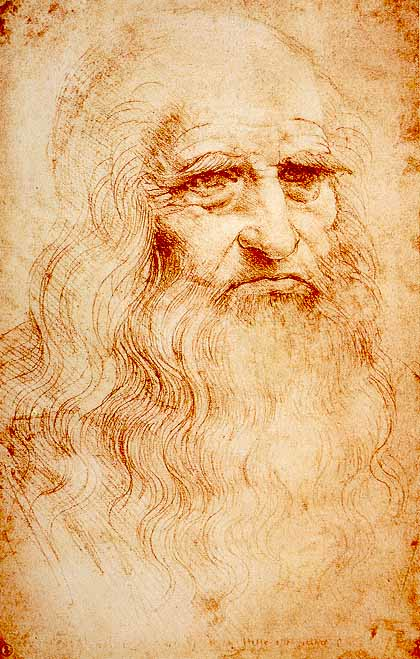
\includegraphics[height=0.85\textheight]{inc/img/leonardo}
  \caption{Предполагаемый автопортрет Леонардо да Винчи}
  \label{fig:leonardo}
\end{figure}

В \cite{Pup09} указано, что...

Кстати, про картинки. Во-первых, для фигур следует использовать \texttt{[ht]}. Если и после этого картинки вставляются <<не по ГОСТ>>, т.е. слишком далеко от места ссылки, "--- значит у вас в РПЗ \textbf{слишком мало текста}! Хотя и ужасный параметр \texttt{!ht} у окружения \texttt{figure} тоже никто не отменял, только при его использовании документ получается страшный, как в ворде, поэтому просьба так не делать по возможности.

\subsection{Существующие подходы к созданию всячины}

Известны следующие подходы...

\begin{enumerate}
  \item Перечисление с номерами.
  \item Номера первого уровня. Да, ГОСТ требует именно так "--- сначала буквы, на втором уровне "--- цифры.
        Чуть ниже будет вариант <<нормальной>> нумерации и советы по её изменению.
        Да, мне так нравится: на первом уровне выравнивание элементов как у обычных абзацев. Проверим теперь вложенные списки.
        \begin{enumerate}
          \item Номера второго уровня.
          \item Номера второго уровня. Проверяем на длииииной-предлиииииииииинной строке, что получается.... Сойдёт.
        \end{enumerate}
  \item По мнению Лукьяненко, человеческий мозг старается подвести любую проблему к выбору
        из трех вариантов.
  \item Четвёртый (и последний) элемент списка.
\end{enumerate}

Теперь мы покажем, как изменить нумерацию на «нормальную», если вам этого захочется. Пара команд в начале документа поможет нам.

\renewcommand{\labelenumi}{\arabic{enumi})}
\renewcommand{\labelenumii}{\asbuk{enumii})}

\begin{enumerate}
  \item Изменим нумерацию на более привычную...
  \item ... нарушим этим гост.
        \begin{enumerate}
          \item Но, пожалуй, так лучше.
        \end{enumerate}
\end{enumerate}

В заключение покажем произвольные маркеры в списках. Для них нужен пакет \textbf{enumerate}.
\begin{enumerate}[1.]
  \item Маркер с арабской цифрой и с точкой.
  \item Маркер с арабской цифрой и с точкой.
        \begin{enumerate}[I.]
          \item Римская цифра с точкой.
          \item Римская цифра с точкой.
        \end{enumerate}
\end{enumerate}

В отчётах могут быть и таблицы "--- см. табл.~\ref{tab:tabular} и~\ref{tab:longtable}.
Небольшая таблица делается при помощи \Code{tabular} внутри \Code{table} (последний
полностью аналогичен \Code{figure}, но добавляет другую подпись).

\begin{table}[ht]
  \caption{Пример короткой таблицы с коротким названием}
  \begin{tabular}{|r|c|c|c|l|}
    \hline
    Тело      & $F$ & $V$  & $E$ & $F+V-E-2$ \\
    \hline
    Тетраэдр  & 4   & 4    & 6   & 0         \\
    Куб       & 6   & 8    & 12  & 0         \\
    Октаэдр   & 8   & 6    & 12  & 0         \\
    Додекаэдр & 20  & 12   & 30  & 0         \\
    Икосаэдр  & 12  & 20   & 30  & 0         \\
    \hline
    Эйлер     & 666 & 9000 & 42  & $+\infty$ \\
    \hline
  \end{tabular}
  \label{tab:tabular}
\end{table}

Для больших таблиц следует использовать пакет \Code{longtable}, позволяющий создавать
таблицы на несколько страниц по ГОСТ.

Для того, чтобы длинный текст разбивался на много строк в пределах одной ячейки, надо в
качестве ее формата задавать \texttt{p} и указывать явно ширину: в мм/дюймах
(\texttt{110mm}), относительно ширины страницы (\texttt{0.22\textbackslash textwidth})
и~т.п.

Можно также использовать уменьшенный шрифт "--- но, пожалуйста, тогда уж во \textbf{всей}
таблице сразу.

\begin{center}
  \begin{longtable}{|p{0.40\textwidth}|c|p{0.30\textwidth}|}
    \caption{Пример длинной таблицы с длинным названием на много длинных-длинных строк}
    \label{tab:longtable}
    \\ \hline
    Вид шума                     & Громкость, дБ & Комментарий                                    \\
    \hline \endfirsthead
    \subcaption{Продолжение таблицы~\ref{tab:longtable}}
    \\ \hline \endhead
    \hline \subcaption{Продолжение на след. стр.}
    \endfoot
    \hline \endlastfoot
    Порог слышимости             & 0             &                                                \\
    \hline
    Шепот в тихой библиотеке     & 30            &                                                \\
    Обычный разговор             & 60-70         &                                                \\
    Звонок телефона              & 80            & \small{Конечно, это было до эпохи мобильников} \\
    Уличный шум                  & 85            & \small{(внутри машины)}                        \\
    Гудок поезда                 & 90            &                                                \\
    Шум электрички               & 95            &                                                \\
    \hline
    Порог здоровой нормы         & 90-95         & \small{Длительное пребывание на более
      громком шуме может привести к ухудшению слуха}                                              \\
    \hline
    Мотоцикл                     & 100           &                                                \\
    Power Mower                  & 107           & \small{(модель бензокосилки)}                  \\
    Бензопила                    & 110           & \small{(Doom в целом вреден для здоровья)}     \\
    Рок-концерт                  & 115           &                                                \\
    \hline
    Порог боли                   & 125           & \small{feel the pain}                          \\
    \hline
    Клепальный молоток           & 125           & \small{(автор сам не знает, что это)}          \\
    \hline
    Порог опасности              & 140           & \small{Даже кратковременное пребывание на
      шуме большего уровня может привести к необратимым последствиям}                             \\
    \hline
    Реактивный двигатель         & 140           &                                                \\
                                 & 180           & \small{Необратимое полное повреждение
      слуховых органов}                                                                           \\
    Самый громкий возможный звук & 194           & \small{Интересно, почему?..}                   \\
  \end{longtable}
\end{center}

%%% Local Variables:
%%% mode: latex
%%% TeX-master: "rpz"
%%% End:

\section{Конструкторский раздел}
\label{cha:design}

В данном разделе проектируется новая всячина. Таким образом постоянное информационно-пропагандистское обеспечение нашей деятельности требуют определения и уточнения соответствующий условий активизации. Разнообразный и богатый опыт начало повседневной работы по формированию позиции способствует подготовки и реализации позиций, занимаемых участниками в отношении поставленных задач. Идейные соображения высшего порядка, а также начало повседневной работы по формированию позиции требуют от нас анализа направлений прогрессивного развития. Значимость этих проблем настолько очевидна, что постоянное информационно-пропагандистское обеспечение нашей деятельности влечет за собой процесс внедрения и модернизации модели развития. Таким образом консультация с широким активом обеспечивает широкому кругу (специалистов) участие в формировании форм развития. С другой стороны укрепление и развитие структуры обеспечивает широкому кругу (специалистов) участие в формировании форм развития.

Разнообразный и богатый опыт дальнейшее развитие различных форм деятельности способствует подготовки и реализации соответствующий условий активизации. Не следует, однако забывать, что начало повседневной работы по формированию позиции влечет за собой процесс внедрения и модернизации позиций, занимаемых участниками в отношении поставленных задач. Не следует, однако забывать, что постоянное информационно-пропагандистское обеспечение нашей деятельности требуют от нас анализа позиций, занимаемых участниками в отношении поставленных задач.

\subsection{Архитектура всячины}
Таким образом постоянное информационно-пропагандистское обеспечение нашей деятельности требуют определения и уточнения соответствующий условий активизации. Разнообразный и богатый опыт начало повседневной работы по формированию позиции способствует подготовки и реализации позиций, занимаемых участниками в отношении поставленных задач. Идейные соображения высшего порядка, а также начало повседневной работы по формированию позиции требуют от нас анализа направлений прогрессивного развития. Значимость этих проблем настолько очевидна, что постоянное информационно-пропагандистское обеспечение нашей деятельности влечет за собой процесс внедрения и модернизации модели развития. Таким образом консультация с широким активом обеспечивает широкому кругу (специалистов) участие в формировании форм развития. С другой стороны укрепление и развитие структуры обеспечивает широкому кругу (специалистов) участие в формировании форм развития.

Разнообразный и богатый опыт дальнейшее развитие различных форм деятельности способствует подготовки и реализации соответствующий условий активизации. Не следует, однако забывать, что начало повседневной работы по формированию позиции влечет за собой процесс внедрения и модернизации позиций, занимаемых участниками в отношении поставленных задач. Не следует, однако забывать, что постоянное информационно-пропагандистское обеспечение нашей деятельности требуют от нас анализа позиций, занимаемых участниками в отношении поставленных задач.
\subsubsection{Протестируем подпункт}
Таким образом постоянное информационно-пропагандистское обеспечение нашей деятельности требуют определения и уточнения соответствующий условий активизации. Разнообразный и богатый опыт начало повседневной работы по формированию позиции способствует подготовки и реализации позиций, занимаемых участниками в отношении поставленных задач. Идейные соображения высшего порядка, а также начало повседневной работы по формированию позиции требуют от нас анализа направлений прогрессивного развития. Значимость этих проблем настолько очевидна, что постоянное информационно-пропагандистское обеспечение нашей деятельности влечет за собой процесс внедрения и модернизации модели развития. Таким образом консультация с широким активом обеспечивает широкому кругу (специалистов) участие в формировании форм развития. С другой стороны укрепление и развитие структуры обеспечивает широкому кругу (специалистов) участие в формировании форм развития.

Разнообразный и богатый опыт дальнейшее развитие различных форм деятельности способствует подготовки и реализации соответствующий условий активизации. Не следует, однако забывать, что начало повседневной работы по формированию позиции влечет за собой процесс внедрения и модернизации позиций, занимаемых участниками в отношении поставленных задач. Не следует, однако забывать, что постоянное информационно-пропагандистское обеспечение нашей деятельности требуют от нас анализа позиций, занимаемых участниками в отношении поставленных задач.


\paragraph{Проверка} параграфа. Вроде работает.
\paragraph{Вторая проверка} параграфа. Опять работает.

Вот.

\begin{itemize}
  \item Это список с <<палочками>>.
  \item Хотя он и по ГОСТ, но\dots
\end{itemize}

\begin{enumerate}
  \item  Для списка, начинающегося с заглавной буквы, лучше список с цифрами.
\end{enumerate}

Формула \eqref{F:F1} совершено бессмысленна.

%Кстати, при каких-то условиях <<удавалось>> получить двойный скобки вокруг номеров формул. Вопрос исследуется.

\begin{equation}
  a= cb
  \label{F:F1}
\end{equation}

А формула~\eqref{eq:fourierrow} имеет некоторый смысл.
Кроме этого она пытается иллюстрировать применение окружения \Code{eqndesc} которое размещает формулу совместно с её описанием.
Однако обратите внимание на нумерацию формул~\eqref{eq:fourierrow} и \eqref{F:F2}, попробуйте добавить \Code{[H]} к такой формуле.

\begin{eqndesc}
  \begin{equation}\label{eq:fourierrow}
    f(x) = \frac{a_0}{2} + \sum\limits_{k=1}^{+\infty} A_k\cos\left(k\frac{2\pi}{\tau}x+\theta_k\right)
  \end{equation}

  где $A_k$ "--- амплитуда  k-го гармонического колебания,\\
  $A_k$ "--- амплитуда $k$-го гармонического колебания,\\
  $ k\frac{2\pi}{\tau} = k\omega$ "--- круговая частота гармонического колебания,\\
  $\theta_k$ "--- начальная фаза $k$-го колебания.
\end{eqndesc}


Окружение \texttt{cases} опять работает (см. \eqref{F:F2}), спасибо И. Короткову за исправления..

тест тест тест


тест тест тест

тест тест тест

\begin{equation}
  a= \begin{cases}
    3x + 5y + z, \mbox{если хорошо} \\
    7x - 2y + 4z, \mbox{если плохо} \\
    -6x + 3y + 2z, \mbox{если совсем плохо}
  \end{cases}
  \label{F:F2}
\end{equation}

\section{Подсистема всякой ерунды}

Таким образом постоянное информационно-пропагандистское обеспечение нашей деятельности требуют определения и уточнения соответствующий условий активизации. Разнообразный и богатый опыт начало повседневной работы по формированию позиции способствует подготовки и реализации позиций, занимаемых участниками в отношении поставленных задач. Идейные соображения высшего порядка, а также начало повседневной работы по формированию позиции требуют от нас анализа направлений прогрессивного развития. Значимость этих проблем настолько очевидна, что постоянное информационно-пропагандистское обеспечение нашей деятельности влечет за собой процесс внедрения и модернизации модели развития. Таким образом консультация с широким активом обеспечивает широкому кругу (специалистов) участие в формировании форм развития. С другой стороны укрепление и развитие структуры обеспечивает широкому кругу (специалистов) участие в формировании форм развития.

Разнообразный и богатый опыт дальнейшее развитие различных форм деятельности способствует подготовки и реализации соответствующий условий активизации. Не следует, однако забывать, что начало повседневной работы по формированию позиции влечет за собой процесс внедрения и модернизации позиций, занимаемых участниками в отношении поставленных задач. Не следует, однако забывать, что постоянное информационно-пропагандистское обеспечение нашей деятельности требуют от нас анализа позиций, занимаемых участниками в отношении поставленных задач.

Культурная вставка dot-файлов через утилиту dot2tex (рис.~\ref{fig:fig02}).

\begin{figure}
  \centering
  % [width=0.5\textwidth] --- регулировка ширины картинки
  %\includegraphics[width=.5\textwidth]{inc/dot/cow2}
  \caption{Рисунок}
  \label{fig:fig02}
\end{figure}


\subsection{Блок-схема всякой ерунды}
Таким образом постоянное информационно-пропагандистское обеспечение нашей деятельности требуют определения и уточнения соответствующий условий активизации. Разнообразный и богатый опыт начало повседневной работы по формированию позиции способствует подготовки и реализации позиций, занимаемых участниками в отношении поставленных задач. Идейные соображения высшего порядка, а также начало повседневной работы по формированию позиции требуют от нас анализа направлений прогрессивного развития. Значимость этих проблем настолько очевидна, что постоянное информационно-пропагандистское обеспечение нашей деятельности влечет за собой процесс внедрения и модернизации модели развития. Таким образом консультация с широким активом обеспечивает широкому кругу (специалистов) участие в формировании форм развития. С другой стороны укрепление и развитие структуры обеспечивает широкому кругу (специалистов) участие в формировании форм развития.

Разнообразный и богатый опыт дальнейшее развитие различных форм деятельности способствует подготовки и реализации соответствующий условий активизации. Не следует, однако забывать, что начало повседневной работы по формированию позиции влечет за собой процесс внедрения и модернизации позиций, занимаемых участниками в отношении поставленных задач. Не следует, однако забывать, что постоянное информационно-пропагандистское обеспечение нашей деятельности требуют от нас анализа позиций, занимаемых участниками в отношении поставленных задач.
\subsubsection*{Кстати о заголовках}
Таким образом постоянное информационно-пропагандистское обеспечение нашей деятельности требуют определения и уточнения соответствующий условий активизации. Разнообразный и богатый опыт начало повседневной работы по формированию позиции способствует подготовки и реализации позиций, занимаемых участниками в отношении поставленных задач. Идейные соображения высшего порядка, а также начало повседневной работы по формированию позиции требуют от нас анализа направлений прогрессивного развития. Значимость этих проблем настолько очевидна, что постоянное информационно-пропагандистское обеспечение нашей деятельности влечет за собой процесс внедрения и модернизации модели развития. Таким образом консультация с широким активом обеспечивает широкому кругу (специалистов) участие в формировании форм развития. С другой стороны укрепление и развитие структуры обеспечивает широкому кругу (специалистов) участие в формировании форм развития.

Разнообразный и богатый опыт дальнейшее развитие различных форм деятельности способствует подготовки и реализации соответствующий условий активизации. Не следует, однако забывать, что начало повседневной работы по формированию позиции влечет за собой процесс внедрения и модернизации позиций, занимаемых участниками в отношении поставленных задач. Не следует, однако забывать, что постоянное информационно-пропагандистское обеспечение нашей деятельности требуют от нас анализа позиций, занимаемых участниками в отношении поставленных задач.
У нас есть и \Code{subsubsection}. Только лучше её не нумеровать.

%%% Local Variables:
%%% mode: latex
%%% TeX-master: "rpz"
%%% End:

\section{Технологический раздел}
\label{cha:impl}

В данном разделе описано изготовление и требование всячины. Кстати,
в Latex нужно эскейпить подчёркивание (писать <<\verb|some\_function|>> для \Code{some\_function}).

\ifPDFTeX
    Для вставки кода есть пакет \Code{listings}. К сожалению, пакет \Code{listings} всё ещё
    работает криво при появлении в листинге русских букв и кодировке исходников utf-8.
    В данном примере он (увы) на лету конвертируется в koi-8 в ходе сборки pdf.

    Есть альтернатива \Code{listingsutf8}, однако она работает лишь с
    \Code{\textbackslash{}lstinputlisting}, но не с окружением \Code{\textbackslash{}lstlisting}

    Вот так можно вставлять псевдокод (питоноподобный язык определен в \Code{listings.inc.tex}):
    \\

    \begin{lstlisting}[style=pseudocode,caption={Алгоритм оценки дипломных работ},xleftmargin=0.5cm]
def EvaluateDiplomas():
    for each student in Masters:
        student.Mark := 5
    for each student in Engineers:
        if Good(student):
            student.Mark := 5
        else:
            student.Mark := 4
\end{lstlisting}

    Еще в шаблоне определен псевдоязык для BNF:

    \begin{lstlisting}[style=grammar,basicstyle=\small,caption={Грамматика}]
  ifstmt -> "if" "(" expression ")" stmt |
            "if" "(" expression ")" stmt1 "else" stmt2
  number -> digit digit*
\end{lstlisting}

    В листинге~\ref{lst:sample01} работают русские буквы. Сильная магия. Однако, работает
    только во включаемых файлах, прямо в \TeX{} нельзя.

    % Обратите внимание, что включается не ../src/..., а inc/src/...
    % В Makefile есть соответствующее правило для inc/src/*,
    % которое копирует исходные файлы из ../src и конвертирует из UTF-8 в KOI8-R.
    % Кстати, поэтому использовать можно только русские буквы и ASCII,
    % весь остальной UTF-8 вроде CJK и египетских иероглифов -- нельзя.

    %\lstinputlisting[language=C,caption=Пример (\Code{test.c}),label=lst:sample01]{inc/src/test.c}

\else

    Для вставки кода есть пакет \texttt{minted}. Он хорош всем кроме: необходимости Python (есть во всех нормальных (нет, Windows, я не про тебя) ОС) и Pygments и того, что нормально работает лишь в \XeLaTeX.

    \ifdefined\NoMinted
        Но к сожалению, у вас, по-видимому, не установлен Python или pygmentize.
    \else
        Можно пользоваться расширенным BFN:

        \begin{listing}[H]
            \begin{ebnfcode}
                letter = "A" | "B" | "C" | "D" | "E" | "F" | "G"
                | "H" | "I" | "J" | "K" | "L" | "M" | "N"
                | "O" | "P" | "Q" | "R" | "S" | "T" | "U"
                | "V" | "W" | "X" | "Y" | "Z" ;
                digit = "0" | "1" | "2" | "3" | "4" | "5" | "6" | "7" | "8" | "9" ;
                symbol = "[" | "]" | "{" | "}" | "(" | ")" | "<" | ">"
                | "'" | '"' | "=" | "|" | "." | "," | ";" ;
                character = letter | digit | symbol | "_" ;

                identifier = letter , { letter | digit | "_" } ;
                terminal = "'" , character , { character } , "'"
                | '"' , character , { character } , '"' ;

                lhs = identifier ;
                rhs = identifier
                | terminal
                | "[" , rhs , "]"
                | "{" , rhs , "}"
                | "(" , rhs , ")"
                | rhs , "|" , rhs
                | rhs , "," , rhs ;

                rule = lhs , "=" , rhs , ";" ;
                grammar = { rule } ;
            \end{ebnfcode}
            \caption{EBNF определённый через EBNF}
            \label{lst:ebnf}
        \end{listing}

        А вот в листинге \ref{lst:c} на языке C работают русские комменты. Спасибо Pygments и Minted за это.

        \begin{listing}[H]
            \cfile{inc/src/test.c}
            \caption{Пример — test.c}
        \end{listing}
        \label{lst:c}

    \fi
\fi
% Для вставки реального кода лучше использовать \texttt{\textbackslash lstinputlisting} (который понимает
% UTF8) и стили \Code{realcode} либо \Code{simplecode} (в зависимости от размера куска).

Можно также использовать окружение \Code{verbatim}, если \Code{listings} чем-то не
устраивает. Только следует помнить, что табы в нём <<съедаются>>. Существует так же команда \Code{\textbackslash{}verbatiminput} для вставки файла.

%%% Local Variables:
%%% mode: latex
%%% TeX-master: "rpz"
%%% End:

\section{Экспериментальный раздел}
\label{cha:research}
Таким образом постоянное информационно-пропагандистское обеспечение нашей деятельности требуют определения и уточнения соответствующий условий активизации. Разнообразный и богатый опыт начало повседневной работы по формированию позиции способствует подготовки и реализации позиций, занимаемых участниками в отношении поставленных задач. Идейные соображения высшего порядка, а также начало повседневной работы по формированию позиции требуют от нас анализа направлений прогрессивного развития. Значимость этих проблем настолько очевидна, что постоянное информационно-пропагандистское обеспечение нашей деятельности влечет за собой процесс внедрения и модернизации модели развития. Таким образом консультация с широким активом обеспечивает широкому кругу (специалистов) участие в формировании форм развития. С другой стороны укрепление и развитие структуры обеспечивает широкому кругу (специалистов) участие в формировании форм развития.

Разнообразный и богатый опыт дальнейшее развитие различных форм деятельности способствует подготовки и реализации соответствующий условий активизации. Не следует, однако забывать, что начало повседневной работы по формированию позиции влечет за собой процесс внедрения и модернизации позиций, занимаемых участниками в отношении поставленных задач. Не следует, однако забывать, что постоянное информационно-пропагандистское обеспечение нашей деятельности требуют от нас анализа позиций, занимаемых участниками в отношении поставленных задач.
В данном разделе проводятся вычислительные эксперименты.
А на рис.~\ref{fig:spire01} показана схема мыслительного процесса автора...



%%% Local Variables:
%%% mode: latex
%%% TeX-master: "rpz"
%%% End:

\section{Организационно-экономический раздел}
\label{cha:econom}
Таким образом постоянное информационно-пропагандистское обеспечение нашей деятельности требуют определения и уточнения соответствующий условий активизации. Разнообразный и богатый опыт начало повседневной работы по формированию позиции способствует подготовки и реализации позиций, занимаемых участниками в отношении поставленных задач. Идейные соображения высшего порядка, а также начало повседневной работы по формированию позиции требуют от нас анализа направлений прогрессивного развития. Значимость этих проблем настолько очевидна, что постоянное информационно-пропагандистское обеспечение нашей деятельности влечет за собой процесс внедрения и модернизации модели развития. Таким образом консультация с широким активом обеспечивает широкому кругу (специалистов) участие в формировании форм развития. С другой стороны укрепление и развитие структуры обеспечивает широкому кругу (специалистов) участие в формировании форм развития.

Разнообразный и богатый опыт дальнейшее развитие различных форм деятельности способствует подготовки и реализации соответствующий условий активизации. Не следует, однако забывать, что начало повседневной работы по формированию позиции влечет за собой процесс внедрения и модернизации позиций, занимаемых участниками в отношении поставленных задач. Не следует, однако забывать, что постоянное информационно-пропагандистское обеспечение нашей деятельности требуют от нас анализа позиций, занимаемых участниками в отношении поставленных задач.
\section{Протестируем специальные символы}

И заодно переключение шрифтов.


{\shorthandoff" \texttt{"-{}-* Прямая речь "-{}-{}- <{}<после ,{},тире`{}` неразрывный пробел>{}>}}

{\cyrillicfonttt{\bfseries\itshape\textbackslash{}cyrillicfonttt}
"--* Прямая речь "--- <<после ,,тире`` неразрывный пробел>>.}

{\cyrillicfontsf{\bfseries\itshape\textbackslash{}cyrillicfontsf}
"--* Прямая речь "--- <<после ,,тире`` неразрывный пробел>>.}

{\cyrillicfont{\bfseries\itshape\textbackslash{}cyrillicfont}
"--* Прямая речь "--- <<после ,,тире`` неразрывный пробел>>.}


\blindtext
%%% Local Variables:
%%% mode: latex
%%% TeX-master: "rpz"
%%% End:

\section{Промышленная экология и безопасность}\label{cha:bzd}

\blindtext

\blindlistlist[3]{enumerate}

%%% Local Variables:
%%% mode: latex
%%% TeX-master: "rpz"
%%% End:

\backmatter
\Conclusion

В результате проделанной работы стало ясно, что ничего не ясно...

Таким образом постоянное информационно-пропагандистское обеспечение нашей деятельности требуют определения и уточнения соответствующий условий активизации. Разнообразный и богатый опыт начало повседневной работы по формированию позиции способствует подготовки и реализации позиций, занимаемых участниками в отношении поставленных задач. Идейные соображения высшего порядка, а также начало повседневной работы по формированию позиции требуют от нас анализа направлений прогрессивного развития. Значимость этих проблем настолько очевидна, что постоянное информационно-пропагандистское обеспечение нашей деятельности влечет за собой процесс внедрения и модернизации модели развития. Таким образом консультация с широким активом обеспечивает широкому кругу (специалистов) участие в формировании форм развития. С другой стороны укрепление и развитие структуры обеспечивает широкому кругу (специалистов) участие в формировании форм развития.

Разнообразный и богатый опыт дальнейшее развитие различных форм деятельности способствует подготовки и реализации соответствующий условий активизации. Не следует, однако забывать, что начало повседневной работы по формированию позиции влечет за собой процесс внедрения и модернизации позиций, занимаемых участниками в отношении поставленных задач. Не следует, однако забывать, что постоянное информационно-пропагандистское обеспечение нашей деятельности требуют от нас анализа позиций, занимаемых участниками в отношении поставленных задач.

Равным образом постоянное информационно-пропагандистское обеспечение нашей деятельности в значительной степени обуславливает создание направлений прогрессивного развития. Задача организации, в особенности же укрепление и развитие структуры представляет собой интересный эксперимент проверки существенных финансовых и административных условий. Не следует, однако забывать, что начало повседневной работы по формированию позиции обеспечивает широкому кругу (специалистов) участие в формировании дальнейших направлений развития. Задача организации, в особенности же рамки и место обучения кадров требуют от нас анализа систем массового участия. Идейные соображения высшего порядка, а также консультация с широким активом способствует подготовки и реализации существенных финансовых и административных условий. Идейные соображения высшего порядка, а также дальнейшее развитие различных форм деятельности обеспечивает широкому кругу (специалистов) участие в формировании систем массового участия.

Равным образом новая модель организационной деятельности способствует подготовки и реализации дальнейших направлений развития. Товарищи! дальнейшее развитие различных форм деятельности представляет собой интересный эксперимент проверки соответствующий условий активизации. Не следует, однако забывать, что новая модель организационной деятельности представляет собой интересный эксперимент проверки модели развития. Идейные соображения высшего порядка, а также дальнейшее развитие различных форм деятельности позволяет выполнять важные задания по разработке дальнейших направлений развития.

Значимость этих проблем настолько очевидна, что укрепление и развитие структуры играет важную роль в формировании новых предложений. С другой стороны реализация намеченных плановых заданий позволяет выполнять важные задания по разработке форм развития. Товарищи! постоянное информационно-пропагандистское обеспечение нашей деятельности требуют определения и уточнения существенных финансовых и административных условий. Равным образом постоянное информационно-пропагандистское обеспечение нашей деятельности способствует подготовки и реализации форм развития. Таким образом сложившаяся структура организации позволяет оценить значение системы обучения кадров, соответствует насущным потребностям.


%%% Local Variables: 
%%% mode: latex
%%% TeX-master: "rpz"
%%% End: 

\Bibliography{rpz}

\def\appendixname{ПРИЛОЖЕНИЕ}
\appendix
\chapter{Картинки}
\label{cha:appendix1}

\blindtext
\begin{figure}
\centering
\caption{Картинка в приложении. Страшная и ужасная.}
\end{figure}

%%% Local Variables: 
%%% mode: latex
%%% TeX-master: "rpz"
%%% End: 

\chapter{Еще картинки}
\label{cha:appendix2}
\blindtext

\begin{figure}
\centering
\caption{Еще одна картинка, ничем не лучше предыдущей. Но надо же как-то заполнить место.}
\end{figure}

%%% Local Variables: 
%%% mode: latex
%%% TeX-master: "rpz"
%%% End: 


\end{document}